% \usepackage[margin=2cm]{geometry}


% \begin{tikzpicture}
\begin{tikzpicture}
\filldraw
(0,0) circle (2pt) node[align=center,below] {$ 0 $} --
(3.81,0) circle (2pt) node[align=center,below] {$ \sigma \approx 0.381 $} -- 
(6.18,0) circle (2pt) node[align=center,below] {$ \tau  \approx 0.618 $} --
(10,0) circle (2pt) node[align=center,below] {$ 1 $};
% \draw[-][very thick] (0,0) -- (1,0);
% \draw [thick] (0,-.1) node[below]{0} -- (0,0.1);
% \draw [thick] (0.381,-.1) node[below]{$ \sigma \approx 0.381 $} -- (0.381,0.1);
% \draw [thick] (0.381,-.1) node[below]{$ \tau \approx 0.618 $} -- (0.618,0.1);
% \draw [thick] (1,-.1) node[below]{1} -- (1,0.1);
\end{tikzpicture}

% \begin{tikzpicture}
% \draw(0,0)--(10,0);
% \foreach \x/\xtext in {1/$ \ sigma $,2/$ \tau1$,4/$ 1$,6/$0$,8/$m$,10/$m+n-1$}
%     \draw(\x,5pt)--(\x,-5pt) node[below] {\xtext};
% \draw[decorate, decoration={brace}, yshift=2ex]  (0,0) -- node[above=0.4ex] {$0$'s}  (2,0);
% \draw[decorate, decoration={brace, mirror}, yshift=2ex]  (10,0) -- node[above=0.4ex] {$l$'s and $0$'s with $l$'s separated by at least two $0$'s}  (4,0);
% \end{tikzpicture}

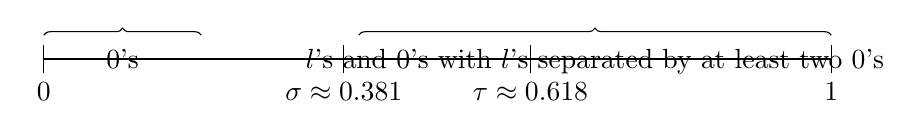
\begin{tikzpicture}
\draw(0,0)--(10,0);
\draw(0,5pt)--(0,-5pt) node[below] {$ 0 $};
\draw(3.81,5pt)--(3.81,-5pt) node[below, align=left] {$ \sigma \approx 0.381 $};
\draw(6.18,5pt)--(6.18,-5pt) node[below, align=left] {$ \tau \approx 0.618 $};
\draw(10,5pt)--(10,-5pt) node[below] {$ 1 $};
\draw[decorate, decoration={brace}, yshift=2ex]  (0,0) -- node[below=0.4ex] {$0$'s}  (2,0);
\draw[decorate, decoration={brace, mirror}, yshift=2ex]  (10,0) -- node[below=0.4ex] {$l$'s and $0$'s with $l$'s separated by at least two $0$'s}  (4,0);
\end{tikzpicture}


\begin{tikzpicture}
\begin{axis}[axis lines=left, xlabel=$x$, ylabel={$f(x)$}, xmin=-5, xmax=5, ymin=0, ymax=5]
\addplot[domain=-10:10,samples=100,color=red]{(x - 2)^2 + 1};
\addlegendentry{$ {(x - 2)}^2 + 1 $}
\addplot[domain=-10:10, samples=100, color=blue]{x^2};
\addlegendentry{$ x^2 $}
\end{axis}
\end{tikzpicture}

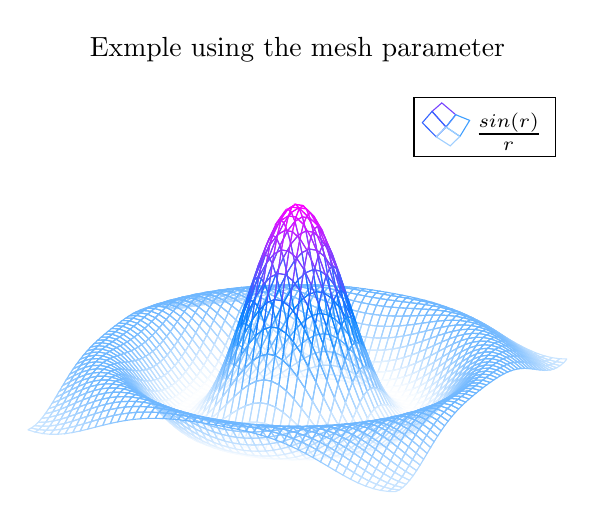
\begin{tikzpicture}
\begin{axis}[
    title=Exmple using the mesh parameter,
    hide axis,
    colormap/cool,
]
\addplot3[
    mesh,
    samples=50,
    domain=-8:8,
]
{sin(deg(sqrt(x^2+y^2)))/sqrt(x^2+y^2)};
\addlegendentry{$\frac{sin(r)}{r}$}
\end{axis}
\end{tikzpicture}

% simple x^2
\begin{tikzpicture}
\begin{axis}[axis lines=left, xlabel=$x$, ylabel={$f(x)$}, xmin=-5, xmax=5, ymin=0, ymax=5]
\addplot[domain=-10:10,samples=100,color=red]{(x - 2)^2 + 1};
\addlegendentry{$ {(x - 2)}^2 + 1 $}
\addplot[domain=-10:10, samples=100, color=blue]{x^2};
\addlegendentry{$ x^2 $}
\end{axis}
\end{tikzpicture}


% triangles
\begin{figure}[H]
\centering
\begin{tikzpicture}

\coordinate[label={150:$A$}] (A) at (135:4);
\coordinate[label={270:$C$}] (C) at (0:0);
\coordinate[label={30:$B$}] (B) at (45:5);
\draw (C) -- (A)node[midway,below left]{$b$} -- (B)  -- cycle node[midway,below right]{$a$};
\draw (C) -- ($(A)!(C)!(B)$) coordinate (P) node[midway,right]{$h$};
\draw[decorate,decoration={brace,raise=12pt,amplitude=5pt}] (A) -- (B);
\path (B) -- (P) node[midway,above]{$x$} -- (A) node[midway,above]{$y$} ($($(A)!0.5!(B)$)!0.8cm!90:(B)$) node{$C$};
\filldraw[fill=white] (C) -- ($(C)!2mm!(A)$) coordinate (U) -- ($(U)!2mm!90:(C)$) --($(C)!2mm!(B)$) --cycle;
\draw ($(P)!2mm!(C)$) coordinate (V) -- ($(V)!2mm!90:(C)$) --($(P)!2mm!(B)$);

\end{tikzpicture}
\caption{Pythagoras}\label{fig:pythagoras} 
\end{figure}
\bigskip


\newcommand\RectTri[4][thick,green!50!black,text=black]{%
\coordinate [label=left:$C$] (C) at #2;
\coordinate [label=below right:$B$] (B) at #3;
\coordinate (aux) at ($ #2 ! 1 ! 90:#3 $);
\coordinate [label=above:$A$] (A) at ($ #2 !#4!(aux) $);

\coordinate (perp) at ($(A)!(C)!(B)$);
\draw[purple!70!black,thick,dashed] (C) -- (perp);

\draw[#1] 
  (C) -- 
  node[auto] {$b$} (A) -- 
  node[auto] {$c$} (B) --
  node[auto] {$a$} 
  (C)
  pic ["$\alpha$",draw,cyan,thick,angle radius=1cm] {angle = C--A--B} 
  pic ["$\alpha$",draw,cyan,thick,angle radius=1cm] {angle = B--C--perp}
  pic ["$\beta$",draw,orange!70!black,thick,angle radius=1cm] {angle = A--B--C}
  pic ["$\beta$",draw,orange!70!black,thick,angle radius=1cm] {angle = perp--C--A};
}

\begin{document}

\begin{tikzpicture}
  \RectTri{(0,3)}{(1,0)}{6cm}
  \begin{scope}[xshift=8.5cm]
    \RectTri[black]{(0,0)}{(4,2)}{4cm}
  \end{scope}
\end{tikzpicture}

\end{document}


\documentclass{article}
\usepackage{tkz-euclide}
\usetkzobj{all}

\begin{document}

\begin{tikzpicture}
  \tkzDefPoint(0,1){A}
  \tkzDefPoint(2,4){C}
  \tkzDefPointWith[orthogonal normed,K=7](C,A)
  \tkzGetPoint{B}

  \tkzLabelPoint[left](A){$A$}
  \tkzLabelPoint[right](B){$B$}
  \tkzLabelPoint[above](C){$C$}

  \tkzMarkRightAngle(A,C,B)

  \tkzDrawSegment[green!60!black](A,C)
  \tkzDrawSegment[green!60!black](C,B)
  \tkzDrawSegment[green!60!black](B,A)

  \tkzLabelSegment[auto](B,A){$c$}
  \tkzLabelSegment[auto,swap](B,C){$a$}
  \tkzLabelSegment[auto,swap](C,A){$b$}

  \tkzDrawAltitude[dashed,color=magenta](A,B)(C)
  \tkzGetPoint{D}

  \tkzMarkAngle[size=1cm,color=cyan,mark=|](C,B,A)
  \tkzMarkAngle[size=1cm,color=cyan,mark=|](A,C,D)
  \tkzMarkAngle[size=0.75cm,color=orange,mark=||](D,C,B)
  \tkzMarkAngle[size=0.75cm,color=orange,mark=||](B,A,C)
\end{tikzpicture}


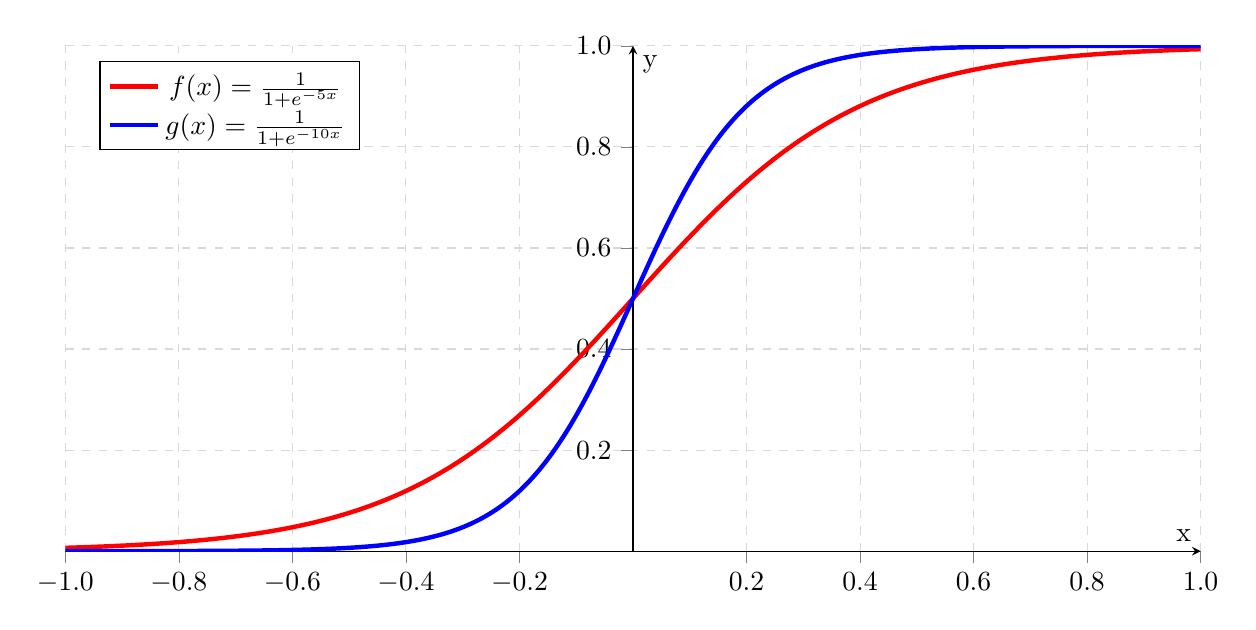
\begin{tikzpicture}
  \begin{axis}[
      legend pos=north west,
      axis x line=middle,
      axis y line=middle,
      x tick label style={/pgf/number format/fixed,
          /pgf/number format/fixed zerofill,
          /pgf/number format/precision=1},
      y tick label style={/pgf/number format/fixed,
          /pgf/number format/fixed zerofill,
          /pgf/number format/precision=1},
      grid = major,
      width=16cm,
      height=8cm,
      grid style={dashed, gray!30},
      xmin=-1,     % start the diagram at this x-coordinate
      xmax= 1,    % end   the diagram at this x-coordinate
      ymin= 0,     % start the diagram at this y-coordinate
      ymax= 1,   % end   the diagram at this y-coordinate
      %axis background/.style={fill=white},
      xlabel=x,
      ylabel=y,
      tick align=outside,
      enlargelimits=false]
    % plot the stirling-formulae
    \addplot[domain=-1:1, red, ultra thick,samples=500] {1/(1+exp(-5*x))};
    \addplot[domain=-1:1, blue, ultra thick,samples=500] {1/(1+exp(-10*x))};
    \addlegendentry{$f(x)=\frac{1}{1+e^{-5x}}$}
    \addlegendentry{$g(x)=\frac{1}{1+e^{-10x}}$}
  \end{axis}
\end{tikzpicture}
\end{document}

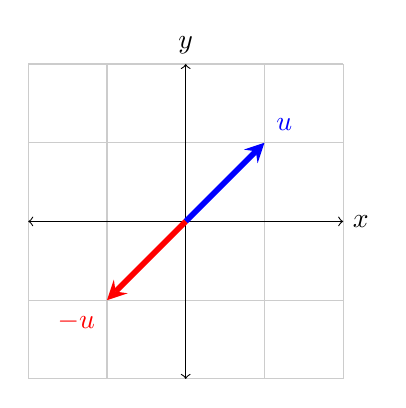
\begin{tikzpicture}
  \draw[thin,gray!40] (-2,-2) grid (2,2);
  \draw[<->] (-2,0)--(2,0) node[right]{$x$};
  \draw[<->] (0,-2)--(0,2) node[above]{$y$};
  \draw[line width=2pt,blue,-stealth](0,0)--(1,1) node[anchor=south west]{$\boldsymbol{u}$};
  \draw[line width=2pt,red,-stealth](0,0)--(-1,-1) node[anchor=north east]{$\boldsymbol{-u}$};
\end{tikzpicture}

\newcommand\plotvectorangle{
  \begin{tikzpicture}
    \draw
    (3,-1) coordinate (a) node[right] {a}
    -- (0,0) coordinate (b) node[left] {b}
    -- (2,2) coordinate (c) node[above right] {c}
    pic["$\alpha$", draw=orange, <->, angle eccentricity=1.2, angle radius=1cm]
      {angle=a--b--c};
  \end{tikzpicture}
}


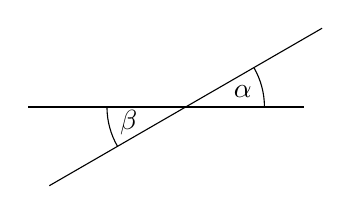
\begin{tikzpicture}
  \draw (-1,0) -- +(3.5,0);
  \draw (1,0) ++(210:2cm) -- +(30:4cm);
  \draw (1,0) +(0:1cm) arc (0:30:1cm);
  \draw (1,0) +(180:1cm) arc (180:210:1cm);
  \path (1,0) ++(15:.75cm) node{$\alpha$};
  \path (1,0) ++(15:-.75cm) node{$\beta$};
\end{tikzpicture}

\[
  f(x) = \left\{
  \begin{array}{ll}
    1 & \text{for } x \in M \\
    0 & \text{for } x \in N
  \end{array}
\]

\[
  \begin{split}
    w_1 + b & > 0 \\
    w_2 + b & > 0 \\
    w_1 + w_2 + b & \le 0 \\
    b & \le 0 \\
  \end{split}
\]

